\section{Potential flow}
\subsection{Incompressible flow}
The idealised fluid in this essay is incompressible. This means that if $\rho$ represents the density of the fluid, then as per definition \ref{definition:INCOMPRESSIBLE}, $\rho$ must 
remain constant over time at every point in the domain of the vector field representing the fluid flow. This means that for any arbitrary closed volume within the fluid, the net mass
flow rate across its boundaries must be zero.

Let the velocity vector field of the fluid $\mathbf{\fatf}$, be defined as $\fatf:x,y\mapsto X(x,y)\ihat+Y(x,y)\jhat$. Then consider an infinitesimal rectangular volume with vertices
$W\point{\alpha_0}{\beta_0}$, $X\point{\alpha_1}{\beta_0}$, $Y\point{\alpha_1}{\beta_1}$ and $Z\point{\alpha_0}{\beta_1}$. Let $\bar{\beta}=\frac{\beta_0+\beta_1}{2}$ and $\bar{\alpha}=\frac{\alpha_0+\alpha_1}{2}$.
Assume $\mathbf{V}$ is continuous and differentiable over this region.

\begin{center}
    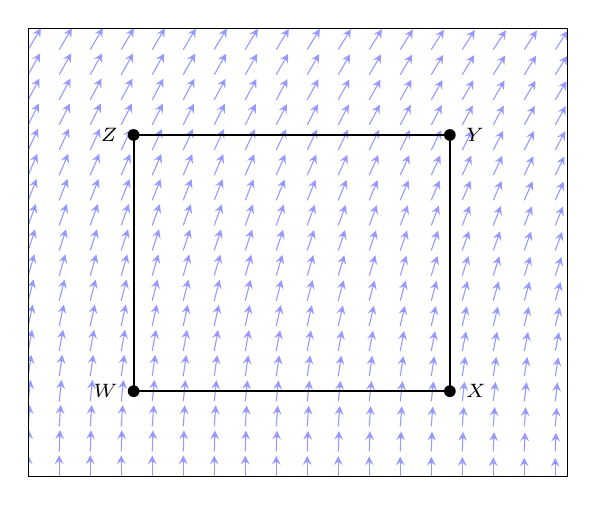
\begin{tikzpicture}[scale=1,X/.style = {circle, fill=black, inner sep=1.5pt,
            label={[font=\scriptsize]left:#1},
            node contents={}},Y/.style = {circle, fill=black, inner sep=1.5pt,
            label={[font=\scriptsize]right:#1},
            node contents={}}]
        \begin{axis}
        [
            domain=0:0.5,
            view={0}{90},
            xtick=\empty,
            ytick=\empty
        ]
        \addplot3[blue, opacity=0.4, quiver={u={sin(deg(y))}, v={cos(deg(x))}, scale arrows=0.025}, -stealth,samples=18] {0};
        \draw[draw=black, thick] (0.1,0.1) rectangle ++(0.3,0.3);
        \draw (0.1,0.1) node[X={$W$}];
        \draw (0.4,0.1) node[Y={$X$}];
        \draw (0.4,0.4) node[Y={$Y$}];
        \draw (0.1,0.4) node[X={$Z$}];
        \end{axis}
    \end{tikzpicture}
\end{center}

Mass is equivalent to density times volume, or mathematically $m=\rho V$, and the derivative of volume with respect to time is
equivalent to the velocity of the fluid elements times the area they flow through, mathematically $\dv{V}{t}=\vec{v}A$. Consequently, the mass flow rate ($\dv{m}{t}$) in to side $WZ$
can be computed as:
$$
    \dv{m}{t}=\rho\dv{V}{t}=m\vec{v}A
$$
Thus along the $x$ axis (in the direction of $\ihat$) the mass flow rate into $WZ$ is given as,
$$
    \rho X(\alpha_0,\bar{\beta})(\beta_1-\beta_0)
$$
and similarly the mass flow rate out of $XY$ is given as:
$$
    \rho X(\alpha_1,\bar{\beta})(\beta_1-\beta_0)
$$
Thus, the net mass flow rate out of the rectangular region along the $x$ axis is:
$$
    \rho X(\alpha_1,\bar{\beta})(\beta_1-\beta_0)-\rho X(\alpha_0,\bar{\beta})(\beta_1-\beta_0)
$$
Which, factoring out $\rho(\beta_1-\beta_0)$, leads to:
$$
    \rho(\beta_1-\beta_0)\left[X(\alpha_1,\bar{\beta})-X(\alpha_0,\bar{\beta})\right]
$$
This by the definition of a partial derivative (because $\alpha_1\rightarrow\alpha_0$) is equivalent to:
$$
    \rho(\beta_1-\beta_0)\eval{\pdv{X}{x}}_{\point{\alpha_0}{\bar{\beta}}}(\alpha_1-\alpha_0)
$$
Analogously, across the $y$ axis, the net mass flow rate out of the rectangular region between sides $WX$ and $ZY$ is given by the expression:
$$
    \rho(\alpha_1-\alpha_0)\eval{\pdv{Y}{y}}_{\point{\bar{\alpha}}{\beta_0}}(\beta_1-\beta_0)
$$
Therefore the net mass flow rate ($\dot{m}$) out of the rectangular region, which must be equal to 0 for the fluid to be incompressible, is given by:
\begin{align*}
    \dot{m}&=\rho(\beta_1-\beta_0)\eval{\pdv{X}{x}}_{\point{\alpha_0}{\bar{\beta}}}(\alpha_1-\alpha_0)+\rho(\alpha_1-\alpha_0)\eval{\pdv{Y}{y}}_{\point{\bar{\alpha}}{\beta_0}}(\beta_1-\beta_0)\\
    &=\rho(\beta_1-\beta_0)(\alpha_1-\alpha_0)\left[\eval{\pdv{X}{x}}_{\point{\alpha_0}{\bar{\beta}}}+\eval{\pdv{Y}{y}}_{\point{\bar{\alpha}}{\beta_0}}\right]=0\\
    \implies0&=\eval{\pdv{X}{x}}_{\point{\alpha_0}{\bar{\beta}}}+\eval{\pdv{Y}{y}}_{\point{\bar{\alpha}}{\beta_0}}
\end{align*}
Then as $\alpha_1\rightarrow\alpha_0$ and $\beta_1\rightarrow\beta_0$, $\bar{\alpha}\rightarrow\alpha_0$ and $\bar{\beta}\rightarrow\beta_0$, meaning
\begin{align*}
    \eval{\pdv{X}{x}}_{\point{\alpha_0}{\beta_0}}+\eval{\pdv{Y}{y}}_{\point{\alpha_0}{\beta_0}}&=0\\
    \therefore\eval{\divergence{\fatf}}_{\point{\alpha_0}{\beta_0}}&=0
\end{align*}
Consequently, as $\point{\alpha_0}{\beta_0}$ is any point in the domain of $\fatf$ where the function is differentiable, the statement can be generalised as:
$$
    \divergence{\fatf}=0
$$

\subsection{Irrotational flow}\label{section:IRROTATIONAL}
As mentioned in definition \ref{definition:VP}, one resulting property of the idealisations (steady, inviscid and incompressible flow)
made in this essay is irrotational flow. If flow is rotational, then there exists points at which $\curl{\fatf}\neq0$. In other words, if one were to
imagine a water wheel at some point in the fluid, and it spins, then the flow is rotational, and vice versa for irrotational flow.
However, flow being irrotational does not imply that it cannot curve, for example $\curl{\fatf}=0$ in cases such as:
\begin{align*}
    &\fatf:x,y\mapsto X(x,y)\ihat+Y(x,y)\jhat\quad\forall\point{x}{y}\neq\point{0}{0}\\
    &X:x,y\mapsto-\frac{y}{x^2+y^2}\,,\quad Y:x,y\mapsto\frac{x}{x^2+y^2}
\end{align*}
Applying the quotient rule to compute the derivatives for both $X$ and $Y$ gives:
\begin{align*}
    \pdv{X}{y}&=-\frac{\left(\pdv{y}y\right)\left(x^2+y^2\right)-y\pdv{y}\left(x^2+y^2\right)}{\left(x^2+y^2\right)^2}\\
    &=-\frac{x^2+y^2-y(2y)}{\left(x^2+y^2\right)^2}\\
    &=-\frac{x^2-y^2}{\left(x^2+y^2\right)^2}
\end{align*}
\begin{align*}
    \pdv{Y}{x}&=\frac{\left(\pdv{x}x\right)\left(x^2+y^2\right)-x\pdv{x}\left(x^2+y^2\right)}{\left(x^2+y^2\right)^2}\\
    &=\frac{x^2+y^2-x(2x)}{\left(x^2+y^2\right)^2}\\
    &=\frac{-x^2+y^2}{\left(x^2+y^2\right)^2}=-\frac{x^2-y^2}{\left(x^2+y^2\right)^2}
\end{align*}
Thus,
\begin{align*}
    \pdv{X}{y}=\pdv{Y}{x}\implies\pdv{Y}{x}-\pdv{X}{y}=0\\
    \therefore\curl{\fatf}=0
\end{align*}
Plotting the vector field for $\fatf$ reveals circulation around the origin, suggesting rotational flow, but which, with a curl of 0 (everywhere except for
the origin, where $\fatf$ is undefined), is irrotational\referto{figure}{figure:ZEROCURL}.
\begin{figure*}[!ht]
    \includegraphics[scale=0.5]{0_curl.pdf}
    \centering
    \caption{The function $\fatf:x,y\mapsto\begin{pmatrix}
        -y\left(x^2+y^2\right)^{-1}\\x\left(x^2+y^2\right)^{-1}
    \end{pmatrix}$ is irrotational despite curving}
    \label{figure:ZEROCURL}
\end{figure*}
\begin{theorem}[Kelvin's theorem]
\end{theorem}

\section{Formulation of the problem}
\section{Governing equations and boundary Conditions}